\documentclass[../main.tex]{subfiles}

\begin{document}
\subsection{The reactive manifesto} As mentioned in the introduction each
today's systems have to handle big loads of data, coming from thousands of
concurrent users, which are demanding low latency responses by terms of
milliseconds and robust systems with a 100\% of up time.

The reactive manifesto \autocite{2014TheManifesto} calls Reactive Systems the
ones able to cope with this expectances and gives this description: "Reactive
Systems are more flexible, loosely-coupled and scalable. This makes them easier
to develop and amenable to change. They are significantly more tolerant of
failure and when failure does occur they meet it with elegance rather than
disaster. Reactive Systems are highly responsive, giving users effective
interactive feedback."

%% Consider talking about https://www.lightbend.com/blog/why-do-we-need-a-reactive-manifesto

At the same time it describes what the traits of reactive systems are. This
traits can be categorised hierarchically by the end goal they serve. Being
responsiveness the trait which directly provides value to systems and the other
three characteristics that reactive systems need to meet in order to be
responsive. This relationship can be visualised in the Figure
\ref{fig:reactive}.

\begin{figure}[ht] \centering
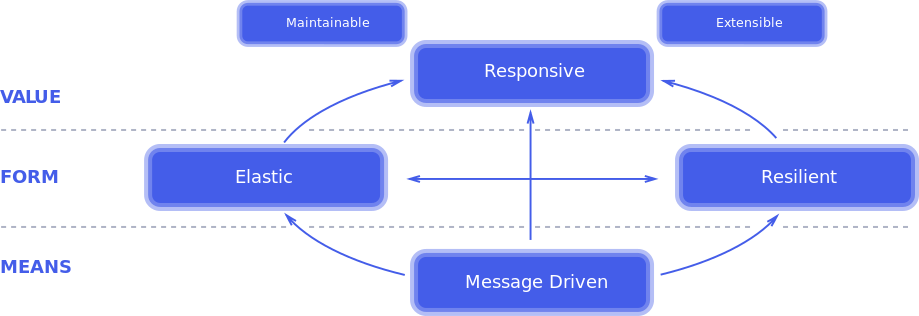
\includegraphics[width=\textwidth]{images/reactive-traits.png}
    \caption{A hierarchical view at the reactive principles.}
    \label{fig:reactive}
\end{figure}

\subsection{The reactive principles}
\subsubsection{Responsive}

Responsiveness is the cornerstone of the reactive
systems. Systems which are responsive are more comfortable to use for users as
they respond faster and adapt quicker to their needs.

Google found out in 2007 that additional 0.5 seconds of load time of a search
could lead to a loss of interest of on the search of a 20\%.
%%https://www.youtube.com/watch?v=BQwAKsFmK_8

More recently in an study developed by Akamai Technologies in 2017 other
insights about consequences of pages responsiveness, being some of the most
interesting.

\begin{itemize}
    \item A 100-millisecond delay in website load time can hurt conversion rates
by 7 percent

    \item A two-second delay in web page load time increase bounce rates by 103
percent

    \item 53 percent of mobile site visitors will leave a page that takes longer
than three seconds to load
\end{itemize}

With that in mind is important to design systems that respond to user request
with low latency in a consistent manner.

At the same responsiveness is about creating systems in which errors can be
detected quickly and dealt effectively.

\subsubsection{Resilient}

Resilience provides a better responsiveness as systems
react better to failure. A resilient system is able to operate even if parts of
it are failing. As an example if a user is using a social network he should be
able to see friends posts if the chat system is unavailable.

At the same time resiliency is the ability to recover from errors without manual
intervention and local errors shouldn't be propagated but rather handled and
managed by different parts of the system.

When designing reactive systems errors should be expected to occur. Even if all
the possible applications errors could be avoided there are other elements of
the applications which are out of control, such as network errors or
interactions with external systems. This principle is stated in the
\textit{Design for failure} approach [[Insert reference ]] which embraces the
acknowledge of possible errors, thus having to make systems which can have
errors but needs to be able to recover from them.

\subsubsection{Elastic}

Applications traffic isn't stable. Online commerces
usually have much higher demands on holidays season like Christmas. A marketing
campaign can create higher traffic than usual in applications. Even an
unexpected reference in a newspaper or a website may increase the number of
users to an unmanageable amount with the original design.

Load balancers or more advanced orchestration systems like Kubernetes
\cite{Production-GradeKubernetes} can handle elasticity on the infrastructure
level, allowing replicas of the application to coexist. However applications
have to be designed to allow the distribution of work among the instances of the
application, this is refered as the Systems scalability.

\paragraph{Scalability}

The Scalability of a system is the capacity that it has to increase its
throughput respectively to its hardware resources. It is defined by the
Universal Law of Computational Scalability [[Insert citation]], the formula
is a variation of the Amhdalh's law [[Insert citation]] and is present in figure \ref{fig:scalability}

\begin{figure}[ht] \centering
  $C(N)={\frac {N}{1+\alpha (N-1)+\beta N(N-1)}}$
  \caption{The Universal Law of Computational Scalability formula}
  \label{fig:scalability}
\end{figure}

In the formula the parameter $N$ represents the amount of concurrent process
running the application. $\alpha$ is the time that is lost because of the need
to wait for shared resources to become available. And $\beta$ the time that
distributed nodes take to have consistent data.

The mere act of increasing the parallelism of an application by adding more
computation nodes doesn't mean that the application will scale linearly to it.
Systems have to be designed in order to use efficiently the computer resources.

\subsubsection{Message driven}

The way to achieve Elastic and Resilient systems is by the use of asynchronous
message passing by this mechanishm application are decoupled both by space
and time.

If modules of the application are communicated by asynchronous messages the end
location of the resource which will handle the message is transparent for the
caller. A message will be delivered to a mailbox. The specific receptor of the
message is not known. A load balancer can choose which will be the recipient of
the message, allowing \textbf{Elasticity}.

As messages are asynchronous the sender of the message doesn't need to wait to a
response of the receiver of it, and can handle other workloads or even terminate
as is no longer responsible of the message.

This decoupling provides greater \textbf{resilience} because the asynchronous
boundary isolate errors from being propagated. Indeed errors can be propagated
as messages, having specific error handler modules which can act in consequence
to avoid the collapse of the system and allow a gracefully recover of failure.
\end{document}